\documentclass[40pt]{article}
\usepackage{mathptmx,amsmath}
\usepackage{pdfslide2}%,pause}
\usepackage[pdftex]{graphicx}
\usepackage[T1]{fontenc} %need for portuguese caracters
\graphicspath{{./figures/}}
\usepackage{float}
\usepackage{tabularx}
\usepackage{braket}

\definecolor{itblue}{rgb}{0.0,0.0,0.5}
\definecolor{itred}{rgb}{0.82,0.18,0.24}
\definecolor{title}{RGB}{68,85,95}
\definecolor{author}{RGB}{120,144,159}

\newcommand{\half}{\textstyle \frac{1}{2}}%
\newcommand{\fig}[2]{\colorbox{white}{\includegraphics[scale=#2]{#1}}}%
%\newcommand{\fig}[2]{\includegraphics[scale=#2]{#1}}%
\newcommand{\pd}[2]{\frac{\partial #1}{\partial #2}}%
\newcommand{\cb}[1]{{\color{itblue} #1}}%
\renewcommand{\labelitemi}{\textcolor{itred}{\normalsize $\bullet$}}
\renewcommand{\labelitemii}{\textcolor{green}{$\star$}}
\newcommand{\ave}[1]{\langle #1 \rangle}%
\newcommand{\mysection}[1]{\section*{\color{black}\sffamily #1}}%

\pagestyle{title}

\begin{document}

%------------TITLE SLIDE -------
\begin{titlepage}  \overlay{it_0.png}

\color{itblue} \sffamily \noindent \normalsize
\hspace*{4cm} Quantum Technologies, 2018/19\\
\hspace*{4cm} Physics Department, University of Aveiro\\
\\
\\
\hspace*{6.5cm}\begin{minipage}{15in}
\vspace*{2cm}
\begin{flushleft}
 \color{title} \sffamily \noindent \Huge
\textbf{Coherent One Way (COW) QKD Protocol}
\end{flushleft}
\end{minipage}
\vspace*{2cm}\\
\\
\hspace*{6.5cm}
%\begin{minipage}{7.5cm}
\color{author}
\Large João António$^1$, Daniel Pereira$^{2,3}$, Armando N. Pinto$^{2,3}$\\
%\end{minipage}\
\\
\vspace*{2cm}\\
\hspace*{6.5cm}
\begin{minipage}{13cm}
\color{title}
\large Physics Department$^1$,\\
Department of Electronics, Telecommunications and Informatics$^2$,\\
University of Aveiro, Aveiro, Portugal\\
Instituto de Telecomunica\c{c}\~{o}es,$^3$, Aveiro, Portugal
\end{minipage}\
\\
\vspace*{2cm}
\\[-1.5mm]
\hspace*{11in}\large \copyright 2018, it - instituto de
telecomunica\c{c}\~{o}es.

\end{titlepage}


%%%%%%%%%%%%%%%%%%%%%%%%%%%%%%%%%%%%
%------------ CONTENT SLIDE -------%
%%%%%%%%%%%%%%%%%%%%%%%%%%%%%%%%%%%%
\headskip=0pt \mysection{\hspace*{2cm} \Huge{Quantum Key Distribution}} \Large
\overlay{it_1.png}
\noindent \\[-5mm]
 \hspace*{.5in}
%\begin{minipage}{15in}
Quantum Key Distribution (QKD) is a secure way of sharing a unique random key (composed of 0 and 1) between two parties spatially distant. They later use this symmetric key to encrypt and decrypt messages between them.

To share/create the random key, they use two channels, one quantum channel and one Authenticated classic channel (can be eavesdropped but can't be modified).

  \begin{figure}[hbt]
    	\centering
    	\includegraphics[width=0.6\textwidth]{./figures/All.pdf}
        	\label{All}
    \end{figure}
%\end{minipage}




%%%%%%%%%%%%%%%%%%%%%%%%%%%%%%
%------------ SLIDE 1 -------%
%%%%%%%%%%%%%%%%%%%%%%%%%%%%%%
\mysection{\Huge Quantum Key Distribution} \Large
\vspace*{1cm}
The two main types of QKD are Polarization protocols and Time Bin protocols.

The Coherent One Way (COW) protocol was elaborated by Nicolas Gisin et al in 2004 [1]. 
Uses time bin properties.

It is also characterized by having a very simple experimental setup since Bob's apparatus is passive.

    \begin{figure}[hbt]
    	\centering
    	\includegraphics[width=0.55\textwidth]{./figures/Alice.pdf}
        	\label{bob}
    \end{figure}

\large
[1] Gisin, Nicolas, et al. "Towards practical and fast quantum cryptography." arXiv preprint quant-ph/0411022 (2004).



%%%%%%%%%%%%%%%%%%%%%%%%%%%%%%
%------------ SLIDE x -------%
%%%%%%%%%%%%%%%%%%%%%%%%%%%%%%
\mysection{\Huge COW - Protocol}\Large
\vspace*{0.3cm}

\begin{description}
  \item[Step 1] Alice creates a random key using:  

$$|0\rangle = |\alpha\rangle |\emptyset\rangle$$      
  $$|1\rangle = |\emptyset\rangle |\alpha\rangle$$
$$|d\rangle = |\alpha\rangle |\alpha\rangle$$

Where $|\emptyset\rangle$ is the vacuum state and $|\alpha\rangle$ is a coherent state of light with intensity $\mu=|\alpha|^2$ and spreads a few random decoy states ($|d\rangle$) in random locations during the creation of the key.
      
  \begin{figure}[hbt]
    	\centering
    	\includegraphics{./figures/Simple.png}
        	\label{Simple}
    \end{figure}

\end{description}


%--------------------------------------------------------------------------------------------------
%------------ SLIDE -------------------------------------------------------------------------------

\mysection{\Huge COW - Protocol}\Large

\begin{description}
  \item[Step 2] Bob's detection is completely passive. An asymmetric coupler sends a fraction $t_B$ of the photons into the data line. That consist of a single photon counter $D_B$, where the bits are discriminated by the time of arrival.

    
    \begin{figure}[hbt]
    	\centering
    	\includegraphics[width=0.6\textwidth]{./figures/Bob.pdf}
        	\label{bob}
    \end{figure}
In the other line half of each pulse interacts with the half of the previous pulse (delayed by 0.5 $T_{bit}$).
\end{description}  


%--------------------------------------------------------------------------------------------------
%------------ SLIDE -------------------------------------------------------------------------------

\mysection{\Huge COW - Protocol}\Large
The $D_{M2}$ (constructive photon counter) should only click when:
\begin{itemize}
\item A logical bit 1 followed by a logical bit 0 where the coherence is across the bit separation (s=1:0);
\item Decoy state where the coherence is within the bit sequence (s=d);
\end{itemize}
All the other photons should click the $D_{M1}$.
  \begin{figure}[hbt]
    	\centering
    	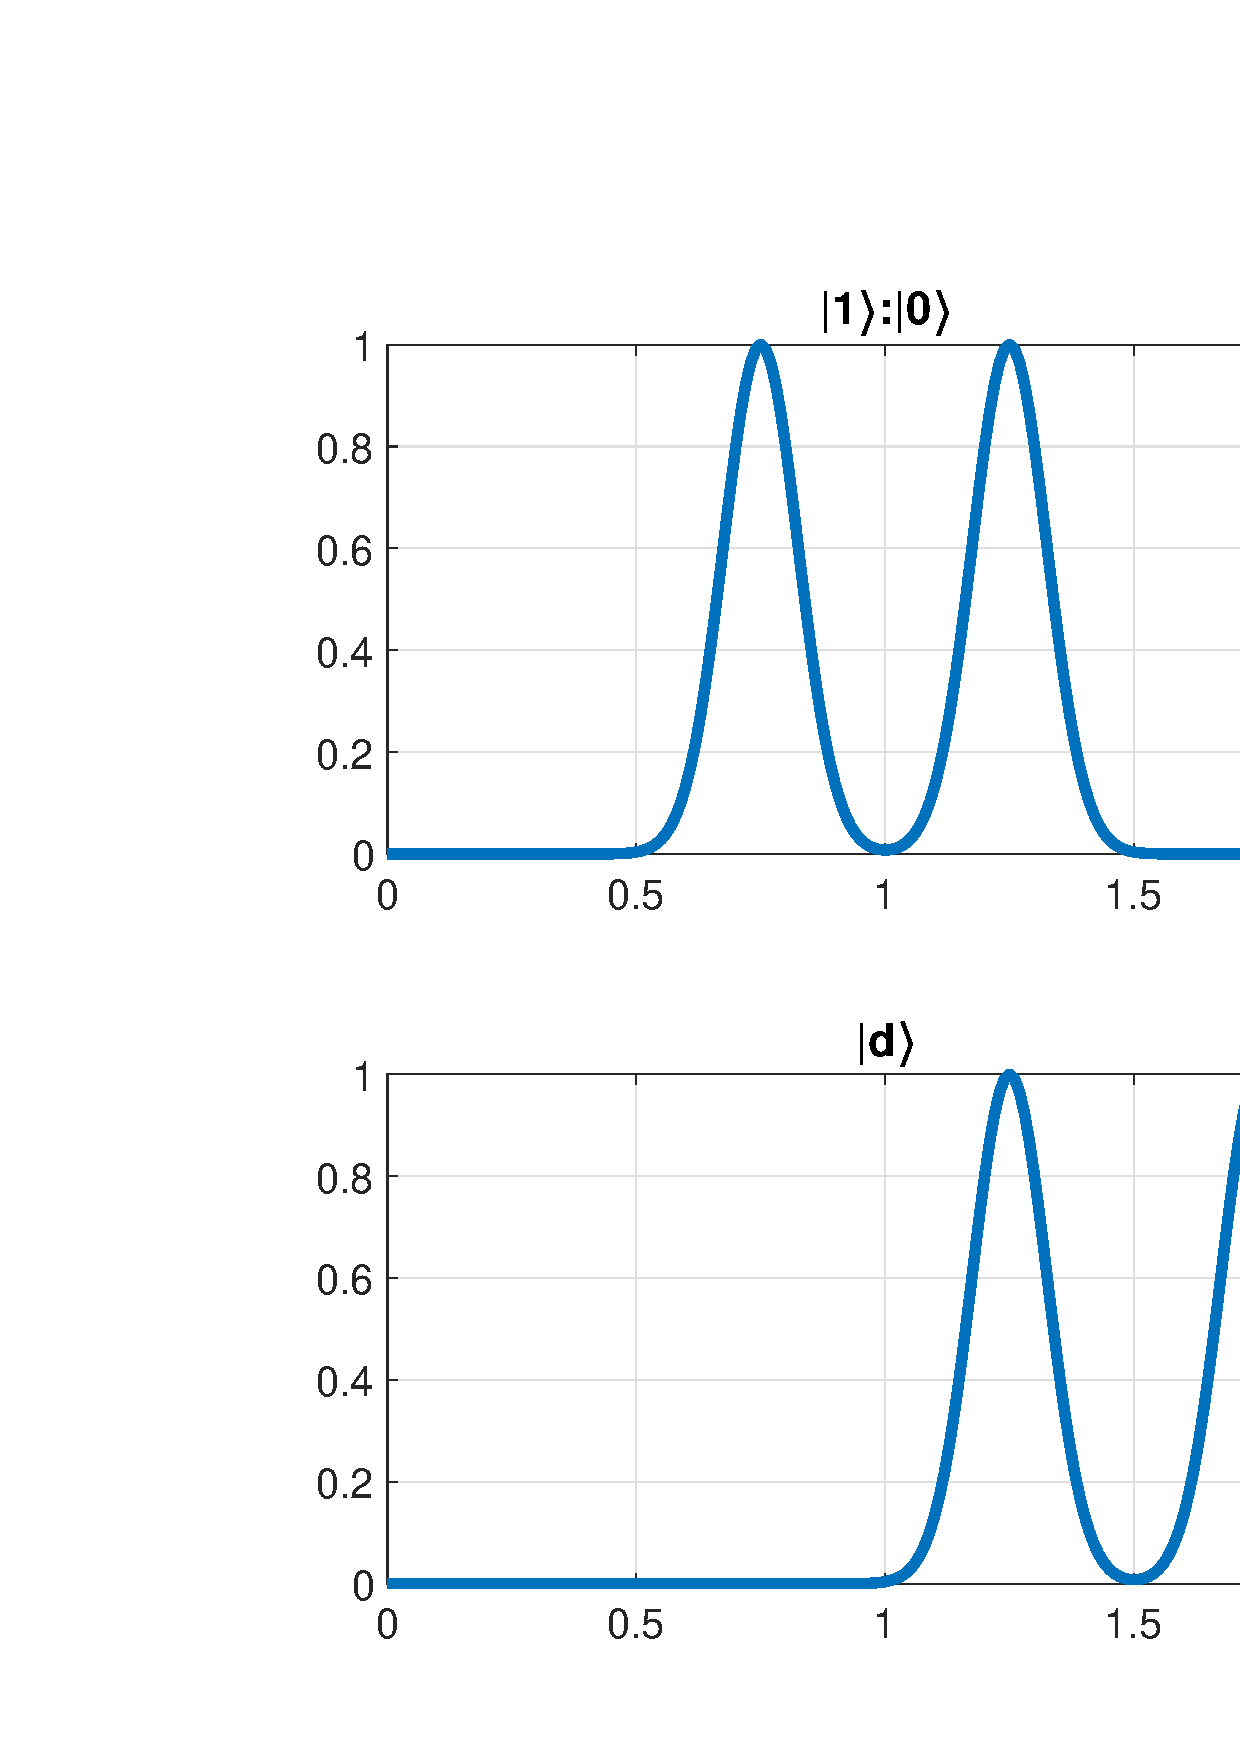
\includegraphics{./figures/Simple2.png}
        	\label{Simple2}
    \end{figure}
%--------------------------------------------------------------------------------------------------
%------------ SLIDE -------------------------------------------------------------------------------

\mysection{\Huge COW - Protocol}\Large
\begin{description}

\item [Step 3] Alice tell Bob the times of the decoy sequences ($2k_d$  \& $ 2k_d-1$). Bob also checks if the $D_{M2}$ has ever fired during a $2k_d$ time. Thus they estimate the break of coherence of decoy pulses.

\item [Step 4] Bob reveals the times that he had a detection in $D_{M2}$, Alice verifies if they belong to a $|1\rangle:|0\rangle$, thus, Alice and Bob estimate the break of coherence across the bit separation.

\item [Step 5] Finally, Bob reveals the items that he has detected in the data line. Alice and Bob run error correction and privacy amplification on these bits and end up with a secret key.

\end{description}


%-------------------------------------------------------------------
%------------ SLIDE ------------------------------------------------
\mysection{} \sffamily \Large
\vspace{-10mm}
\centerline{E-mail: joaoantonio@ua.pt}
\vspace*{7cm}
\begin{itemize}
	\item Gisin, Nicolas, et al. "Towards practical and fast quantum cryptography." arXiv preprint quant-ph/0411022 (2004).
	\item Branciard, Cyril, et al. "Zero-error attacks and detection statistics in the coherent one-way protocol for quantum cryptography." arXiv preprint quant-ph/0609090 (2006).
	\item Kronberg, Dmitry Anatol'evich, et al. "Analysis of coherent quantum cryptography protocol vulnerability to an active beam-splitting attack." Quantum Electronics 47.2 (2017): 163.
	\item Roberts, George L., et al. "Modulator‐Free Coherent‐One‐Way Quantum Key Distribution." Laser \& Photonics Reviews 11.4 (2017): 1700067.
\end{itemize}


\end{document}
